
%
% Draft  document dpcpoisson.tex
% Understanding the check effect on fibre diameter
%
 
\documentclass[titlepage]{article}  % Latex2e
\usepackage{graphicx,lscape,subfigure}
\usepackage{tikz}
\usepackage{bm,longtable}
\usepackage{textcomp}
 

\title{Can we convert between observed or {\em checked} diameter and potential or {\em base} diameter?}
\author{Paul Swan, Neville Jackson and Philip Moore}
\date{25 Nov 2021} 

 
\begin{document} 


 
\maketitle      
\tableofcontents

$\newcommand{\E}{\mathrm{E}}$
$\newcommand{\Var}{\mathrm{Var}}$
$\newcommand{\Cov}{\mathrm{Cov}}$ 
$\newcommand{\SD}{\mathrm{SD}}$ 

\clearpage
\section{Introduction} 


Given that the number of cells in each follicle papilla cell aggregate determines the {\em base} or potential diameter of each fibre, and given that we have an empirical equation relating dermal papilla cell number to {\em checked} fibre diameter, we need to see whether we can modify that equation to estimate base or potential fibre diameter.

We need a definition of terms
\begin{description}
\item[fibre cross section area $A$] is calculated from measured fibre diameter as $\frac{\pi}{4}D^{2}$ where $D$  is measured fibre diameter
\item[follicle density] is the count of primary and secondary follicles per unit area of skin as measured on skin biopsies
\item[base diameter] is the maximum or potential diameter that a fibre can grow to given unlimited nutrients and no sharing with surrounding follicles. It is determined by the number of dermal papilla cells in the follicle bulb.  It is actually cross sectional area that is determined, not diameter.  The nearest thing to base diameter or cross sectional area which could be observed would be the diameter of fibres in the sickle tips of primary central follicles as seen in the hairy tips of the birthcoat. These sickle tips are grown {\em in utero} with presumably unrestricted nutrition and are groewn from Pc follicles before any other follicles deveop around them.
\item[checked diameter] is the observed diameter of a fibre under normal conditions of limited nutrients and a certain density of surrounding follicles. 
\end{description}
If we call the observed diameter at time $i$ $D_{i}$ and the base diameter for the same follicle $D_{B}$, then the amount of {\em check} at time $i$ is $\frac{D_{B} - D_{i}}{D_{B}}$. We really should define this in terms of $A$ rather than $D$, so $\frac{A_{B} - A_{i}}{A_{B}}$ is preferable. So check is the fractional reduction in $A_{i}$ below $A_{B}$

What we are setting out to do  is , given $A_{i}$ can we devise a way of estimating $A_{B}$. Clearly some other information such as nutritional level and follicle densities will be needed. 


\clearpage
\section{Materials and Methods}
We utilize data from Carter(1968)~\cite{cart:68} specifically breed means for follicle density and fibre cross sectional area estimated as $A = \frac{\pi}{4}Dps^{2}$. Each mean represents around 20 animals sampled and Dr Carter has stated that all sheep sampled were in good nutritional condition,  and the samplings were mostly at around 2 years of age, ie adult sheep.  A critical aspect is that the diameters and follicle densities were at the same time, ie at the time the skin biopsies were taken.

We also examine various nutrition experiment data sets, some unpublished, in which we have either
\begin{itemize}
\item Sheep subjected to a series of nutritional treatments over time. These types of study are paired comparisons - the same sheep being observed under more than one nutritional regime. They are subject to correlated errors issues because the results for each sheep are a time series. That is unlikely to concern us here.
\item Random samples of sheep are subjected to different nutritional regimes. These studies are randomized block experiments. They depend on having sufficient sheep for random samples to be equivalent in mean.
\end{itemize}
Again the critical requirement was fibre diameter and follicle density measurements at the same time.
 
We also utilize data from Jackson and Downes(1979)~\cite{jack:79} on staple diameter profiles. In these data we only have a follicle density measurement for adult sheep, not at all 10 diameter positions along the staple.

We also utilize data from CSIRO flocks for genetic analysis of fibre diameter and follicle density. Again these had to be either skin section data, or 'cast' technique data, to ensure diameters and follicle densities were concurrent.
\clearpage
\section{Results}

Our fibre diameters calculated from papilla cell counts (Swan, Jackson and Moore(2021)~\cite{swan:21}), and also all observed fibre diameter data, are a {\em checked} fibre diameter. That is, we have been simulating diameters at the average level of {\em check} obtaining in the dataset used to estimate the diameter on papilla cell count regression equation. We do not know quantitatively how much this {\em check} is, but it is substantial - something like $50$ percent of the {\em base} or potential diameter. 

\subsection{What causes check?}
We need to develop some concept of what causes {\em checks} in fibre diameter. We are trying to model a situation where there is a nominal amount of {\em skin nutrients} to be shared between a number of follicles. We are not sure whether the sharing depends on follicle density ( ie follicles per unit skin area), or whether the sharing is within trio groups and depends on intra-group follicle density  or on follicles per group or on group area. We will start with the simple assumption of density dependence regardless of trio groups. For this we can write
\begin{displaymath}
A = k/N
\end{displaymath}
where
\begin{description}
\item[A] is fibre cross sectional area
\item[N] is follicle density
\item[k] is a constant of proportion, somehow related to the amount of skin nutrients
\end{description}
We should note that this proposes an hyperbolic relationship between $A$ and $N$ , ie $AN = k$ is the equation of an hyperbola with asymptotes at the axes. 

That is indeed what is observed. We can revisit the Carter(1968)~\cite{cart:68} data to verify it. These data are particularly valuable because the diameters ( on which cross sectional area is based) and densities were both measured on skin sections and are therefore at the same point in timne.  Figure~\ref{fig:carternxc} shows follicle density plotted against cross sectional area. The data are breed means from around 20 animals per breed sampled.
%\documentclass{article}
%\usepackage{graphicx,subfigure}
%\begin{document}

\begin{figure}[h]
  \centering
   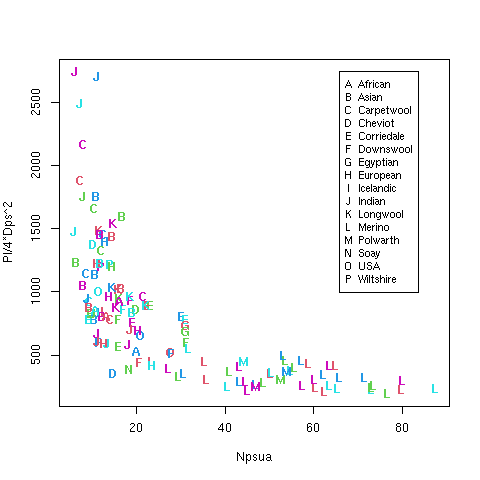
\includegraphics[width=0.9\textwidth]{cartercsaxn.png}
  \caption{Plot of breed means for follicle density and fibre cross sectional area from Carter(1968)~\cite{cart:68}}
  \label{fig:carternxc}
\end{figure}

%\end{document}


There is also the study of Scobie {\em et al}(20..) which demonstrates that the relationship between diameter and density is curvilinear, but does not propose that it is hyperbolic.

The hyperbolic nature of the relationship is apparent. This can be conclusively demonstrated by showing that the data can be linearized with a simple reciprocal transformation of the follicle densities. Figure~\ref{fig:carter1ovnxcreg} shows the reciprocal of follicle density plotted against fibre cross sectional area for the same breed means as in Figure~\ref{fig:carternxc}
%\documentclass{article}
%\usepackage{graphicx,subfigure}
%\begin{document}

\begin{figure}[h]
  \centering
   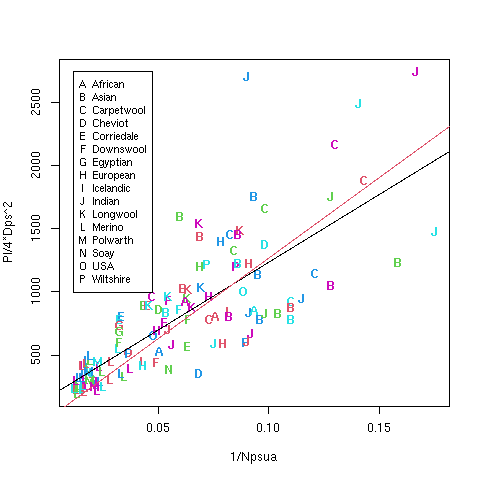
\includegraphics[width=0.9\textwidth]{cartercsax1ovnreg.png}
  \caption{Plot of breed means for reciprocal of follicle density and fibre cross sectional area from Carter(1968)~\cite{cart:68}. The black line is a linear regression fitted with an intercept. The red line is a linear regression fitted without an intercept.}
  \label{fig:carter1ovnxcreg}
\end{figure}

%\end{document}


There is some spread of points but no evidence of curvature. The linear regression without an intercept was $A = 12689 (1/N)$ and had a multiple correlation of $0.87$.  The linear regression with an intercept was $A = 163 + 10700 (1/N)$ and had a multiple correlation of $0.61$. If there is a nonzero intercept it simply means the hyperbola is asymptotic to $A = 163$ instead of to $A = 0$. There seems to be little case for a non zero asymptote.

However the data in Figure~\ref{fig:carter1ovnxcreg} do seem to split into two groups. There may be a case for two regression lines, ie two values of the $k$ constant. This is explored in Figure~\ref{fig:carter1ovnxc2reg}
%\documentclass{article}
%\usepackage{graphicx,subfigure}
%\begin{document}

\begin{figure}[h]
  \centering
   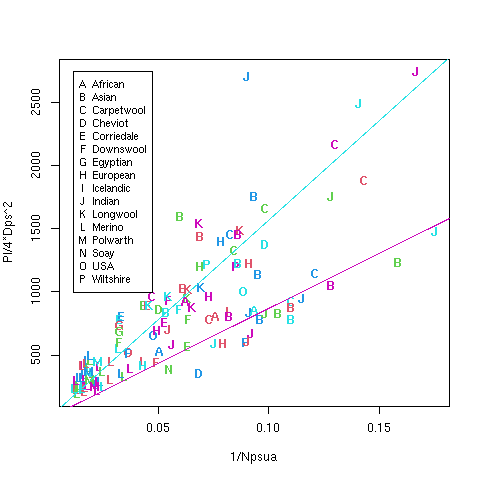
\includegraphics[width=0.9\textwidth]{cartercsax1ovn2reg.png}
  \caption{Plot of breed means for reciprocal of follicle density and fibre cross sectional area from Carter(1968)~\cite{cart:68}. The blue line is a linear regression fitted with a slope of $15689$ and no intercept. The red line is a linear regression fitted with a slope of 8689 and no intercept.}
  \label{fig:carter1ovnxc2reg}
\end{figure}

%\end{document}


So these data exhibit a range of values for $k$ from around 8000 to around 15000 with a mean of 12689. There are two possible reasons that $k$ would vary
\begin{description}
\item[dermal papilla cell number] may vary between breeds. So the maximum potential cross sectional area of fibres may vary. On second thought, this should not affect $k$. Changes in papilla cell  number should simply move the data points along the regression line without changing its slope $k$.
\item[nutrition] of the skin at time of sampling may vary between breeds. So the degree of nutritional check may vary. This is what we are hoping $k$ will be a measure of.
\end{description}

We can even compute an estimate of the value of $k$ for each breed as $k = AN$.  This has a physical interpretation - it is the sum of the cross sectional areas of all fibres in a square millimeter. But it is not the physical interpretation that we are interested in. We see $k$ as an index of nutritional status, provided we can find a way to remove the influences of papilla cell number and density from it. 

\subsection{Identifying the causes of {\em check}}
With the data from Carter(1968)~\cite{cart:68} in the previous section we have been able to demonstrate the reciprocal density component of check in terms of its effect on fibre cross sectional area, but we were left with a value $k$ which could be either a skin nutritional component or could reflect some other unidentified factor.  To try and identify these we need data with a controlled systematic nutritional effect, as in an experiment with various levels of nutrition.

\subsubsection{Daly and Carter experiments}
Daly and Carter(1955)~\cite{daly:55} and (1956)~\cite{daly:56} conducted a series of 3 experiments with Lincoln, Corriedale, Polwarth and Fine Merino ewes. Experiments 1 and 2 were with hand feeding starting with {\em ad lib} for a period of 50 weeks in experiment 1, and moving stepwise down to 20{\em percent} of {\em ad lib} over a period of 30 weeks in experiment 2. Experiment 3 was the same breeds at pasture over a period of 40 weeks during which there was a steady gain in liveweight. The raw data are available in the above publications as Breed means at the starting and ending periods of each experiment, representing good nutrition in experiment 1, good changing to poor nutrition in experiment 2, and the reverse in experiment 3.

The relationship of fibre cross sectional area to the reciprocal of density is shown for experiment 1 in Figure~\ref{fig:dcexpt1reg}
%\documentclass{article}
%\usepackage{graphicx,subfigure}
%\begin{document}

\begin{figure}[h]
  \centering
   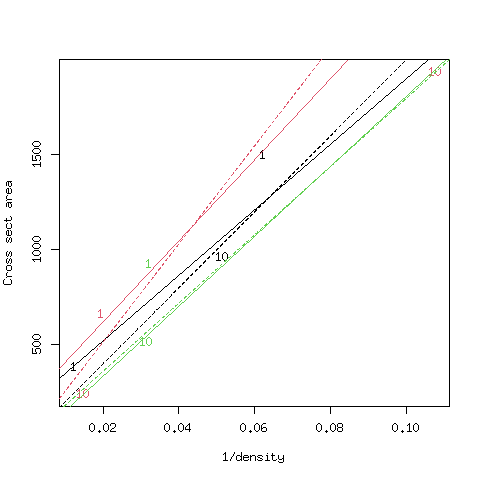
\includegraphics[width=0.9\textwidth]{DC1955/expt1reg.png}
  \caption{Plot of breed means for reciprocal of follicle density and fibre cross sectional area from Daly and Carter(1955)~\cite{daly:55} experiment 1. The black lines are linear regressions fitted to all data, full line with an intercept, dashed line without an intercept. The red lines are linear regressions fitted to breed means for period 1 . The green lines are linear regressions fitted to breed means for period 10 .}
  \label{fig:dcexpt1reg}
\end{figure}

%\end{document}


There is no case for including an intercept. Analyses of variance show that only the regression slopes are significant. We will only discuss results for regressions thru zero.  The estimated slope for Period 1 data was $25837$ (units are microns squared x no of follicles per mm squared). The estimate of slope for Period 10 data was $17941$. The standard errors for these slopes were 1773 and 302 respectively. The difference is significant. These slopes are our estimates of $k$ for for growing animals on {\em ad lib} . So $k$ is larger for younger smaller  animals . 

 The relationship of fibre cross sectional area to the reciprocal of density is shown for experiment 2 in Figure~\ref{fig:dcexpt2reg}
%\documentclass{article}
%\usepackage{graphicx,subfigure}
%\begin{document}

\begin{figure}[h]
  \centering
   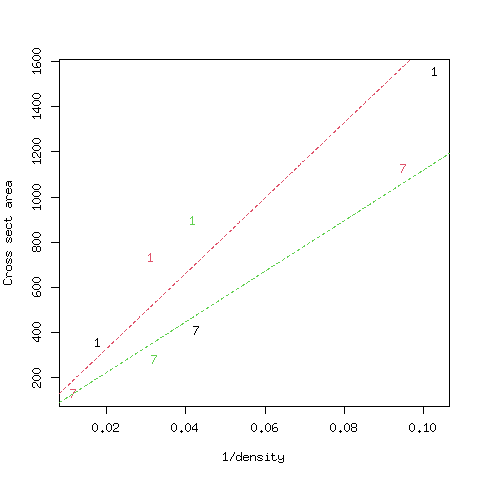
\includegraphics[width=0.9\textwidth]{DC1955/expt2reg.png}
  \caption{Plot of breed means for reciprocal of follicle density and fibre cross sectional area from Daly and Carter(1955)~\cite{daly:55} experiment 2.  The red lines are linear regressions  with zero intercept fitted to breed means for period 1 ({\em ad lib} nutrition. The green lines are linear regressions with zero intercept fitted to breed means for period 7 (restricted nutrition).}
  \label{fig:dcexpt2reg}
\end{figure}

%\end{document}


Here we have a larger difference in slopes but a poorer fit. The red line (good nutrition) is a larger slope than the green line (restricted nutrition). The slopes are $16589$ for Period 1 (good nutrition) and 11159 for Period 7 (poor nutrition). The standard errors are 1670 and 2401 respectively. The difference is again significant.

The $k$ values in experiment 2 are lower than those in experiment 1. The diets in the two experiments were similar, but the sheep were older and of considerably larger LiveWeight in experimant 2. So the absolute value of $k$ does not inform us about level of nutrition, for example $k=17000$ in experiment 1 is a restricted feeding, but $k=17000$ in experiment 2 is an {\em ad lib} feeding. Differences in $k$ mean something in relation to nutrition, other things being equal, but absolute values of $k$ do not indicate level of nutrition. 

Another point of concern in experiment 2 is that the fibre diameters may have been on wool samples, not skin biopsies. The fibre cross sectional areas presented do not agree with what we calculate using the formula $A = \frac{\pi}{4} D^{2}$. They are close but not identical.  We used their fibre cross sectional areas.

There was a third experiment by Daly and Carter using the same sheep as in experiments 1 and 2, but grazed at pasture over a period of 40 weeks. Over the 40 weeks Liveweights rose to a peak at about 30 weeks, then declined slightly as the pasture hayed off in Summer. The relationship of fibre cross sectional area to the reciprocal of density is shown for experiment 3 in Figure~\ref{fig:dcexpt3reg}
%\documentclass{article}
%\usepackage{graphicx,subfigure}
%\begin{document}

\begin{figure}[h]
  \centering
   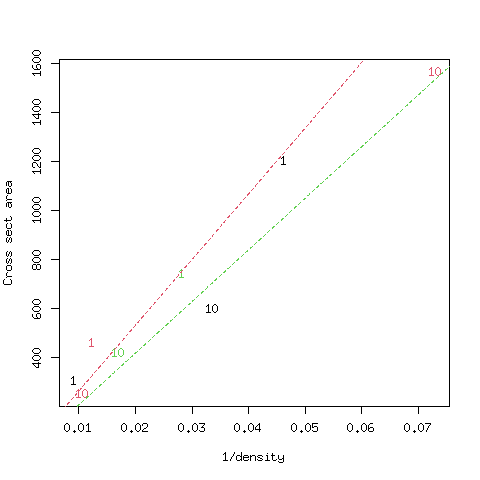
\includegraphics[width=0.9\textwidth]{DC1955/expt3reg.png}
  \caption{Plot of breed means for reciprocal of follicle density and fibre cross sectional area from Daly and Carter(1956)~\cite{daly:56} experiment 3.  The red lines are linear regressions  with zero intercept fitted to breed means for period 1 (lowest liveweight). The green lines are linear regressions with zero intercept fitted to breed means for period 10 (higher liveweight and older).}
  \label{fig:dcexpt3reg}
\end{figure}

%\end{document}


Here, the $k$ value for period 1 was $26768$ and for period 10 was $21004$. Bot $k$ values are high compared to experiments 1 and 2, and the difference is small. Subtle pasture changes do not produce the same dramatic effect as changes in level of hand feeding. The difference is in the expected direction - ie the higher quality pasture of period 1 produced a higher $k$ value than the lower quality pasture of period 10, even though the liveweights increased from period 1 to period 10.

Finally we need to see if shifting scales are an issue by plotting all 3 experiments on one graph. Figure~\ref{fig:dc123} shows this
%\documentclass{article}
%\usepackage{graphicx,subfigure}
%\begin{document}

\begin{figure}[h]
  \centering
   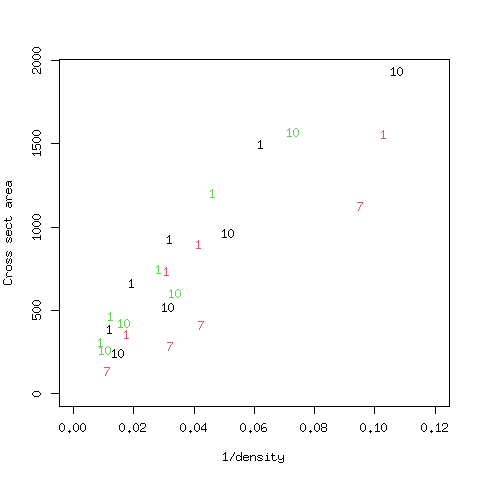
\includegraphics[width=0.9\textwidth]{DC1955/dc123.png}
  \caption{Plot of breed means for reciprocal of follicle density and fibre cross sectional area from Daly and Carter(1956)~\cite{daly:56}  all 3 experiments .  The black points are experiment 1, the red points are experiment 2, the green points are experiment 3.}
  \label{fig:dc123}
\end{figure}

%\end{document}


We can see that there is no shift of scale between experiments. The only really different set of points is period 7 in experiment 2, which had a very low $k$ value of $11159$. It seems visually from Figure~\ref{fig:dc123} that $k$ does not vary greatly.  That is because it is difficult to judge slopes visually. If we calculate $k$ for each Breed x Period x Experimant combination and do an analysis of variance we get
\begin{verbatim}
            Df    Sum Sq   Mean Sq F value   Pr(>F)    
Breed        3  80429331  26809777   2.812   0.0751 .  
Expt         2 540764086 270382043  28.359 8.01e-06 ***
Expt:Period  3 646855973 215618658  22.615 8.06e-06 ***
Residuals   15 143011782   9534119                     
---
Signif. codes:  0 ‘***’ 0.001 ‘**’ 0.01 ‘*’ 0.05 ‘.’ 0.1 ‘ ’ 1
\end{verbatim}
So there are large differences in $k$ between Experiments, and between Periods within Experiments, but there are no Breed differences in $k$ . That is what we concluded doing things one experiment at a time above.  The Breed differences in diameter are due to the density part of the check effect and/or the dermal papilla cell counts. Differences in diameter due to $k$ are to do with growth and development and nutritional status.

\clearpage
\subsubsection{Old unpublished Carter experiments}
A further source of such data is again Dr Carter. Figure~\ref{fig:carterup1} shows an original data sheet of a very old nutritional experiment obtained from Dr Carter in a personal communication. 
%\documentclass{article}
%\usepackage{graphicx,subfigure}
%\begin{document}

\begin{figure}[h]
  \centering
   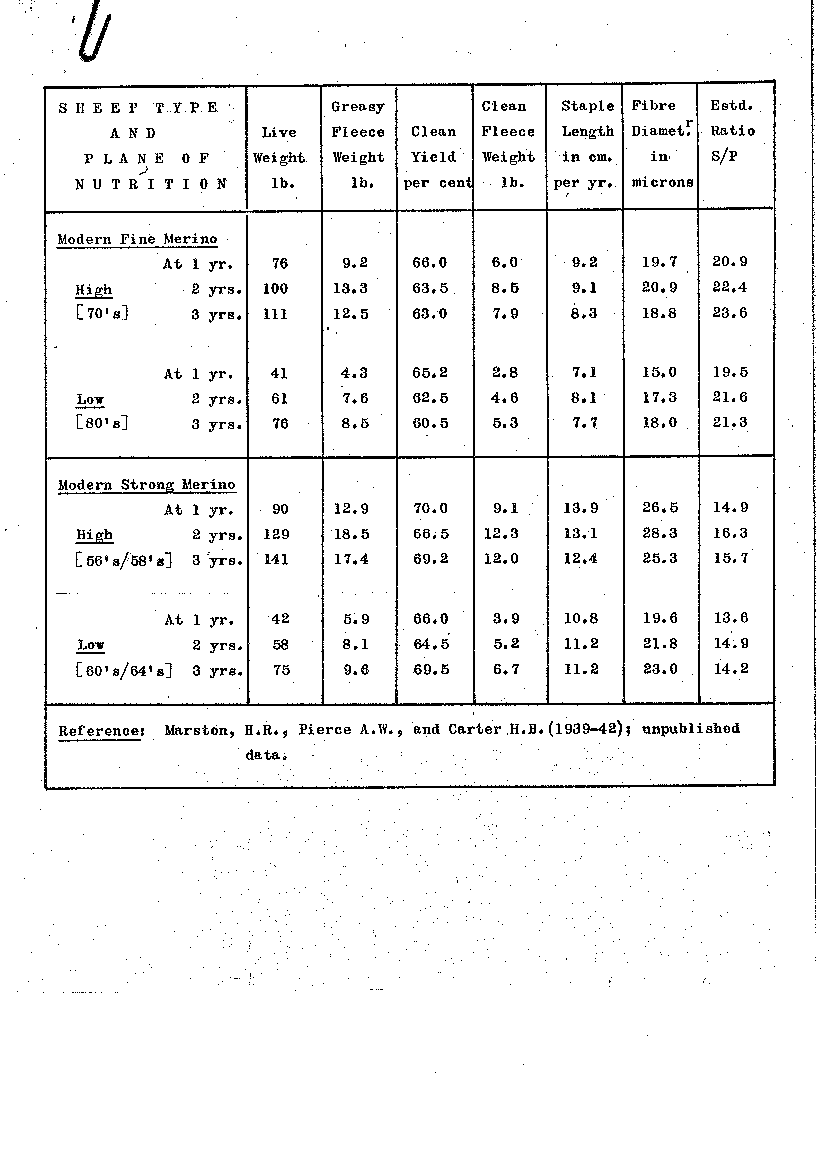
\includegraphics[width=1.1\textwidth]{carterup1.png}
  \caption{Data from an old nutritional experiment obtained from Dr Carter}
  \label{fig:carterup1}
\end{figure}

%\end{document}


This looks promising, there are two planes of nutrition, but the fibre diameter measurement may not be at one point of growth ( ie a skin measurement) , and the 'estimated' S/P ratio is the nearest thing we have to a density. There is a second sheet (Figure~\ref{fig:carterup1a})
%\documentclass{article}
%\usepackage{graphicx,subfigure}
%\begin{document}

\begin{figure}[h]
  \centering
   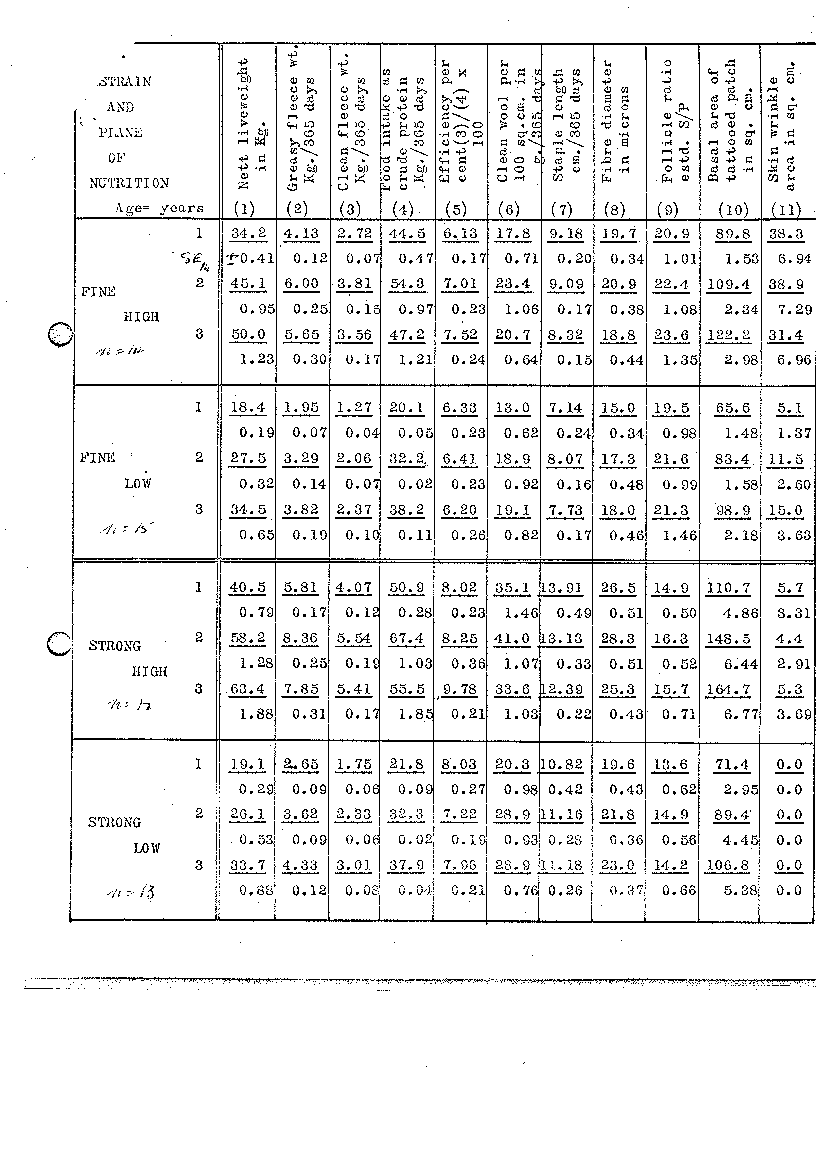
\includegraphics[width=1.1\textwidth]{carterup1a.png}
  \caption{Data from an old nutritional experiment obtained from Dr Carter}
  \label{fig:carterup1a}
\end{figure}

%\end{document}


where sheep numbers have been written in. So it is a randomised design, not a paired design with the same sheep subjected to different nutritional planes at different times. Paired or time series designs are difficultto interpret for our purpose, because nutritional differences at a series of times are confounded with effects of increasing age  and accompanying growt and development of the sheep. For example, if bodyweights increase with age, densities will decrease with age.

For Carters experiment,we can estimate a density from S/P ratio and LiveWeight using $N = 36.7 - 0.714 LiveWt(Kg) + 2.72S/P$ . This formula was obtained from The Daly and Carter data above.
Using this estimated density, and using the 'dubious' fibre diameter to estimate cross sectional area, we obtain the plot of reciprocal density against cross sectional area shown in Figure~\ref{fig:oldcart1}
%\documentclass{article}
%\usepackage{graphicx,subfigure}
%\begin{document}

\begin{figure}[h]
  \centering
   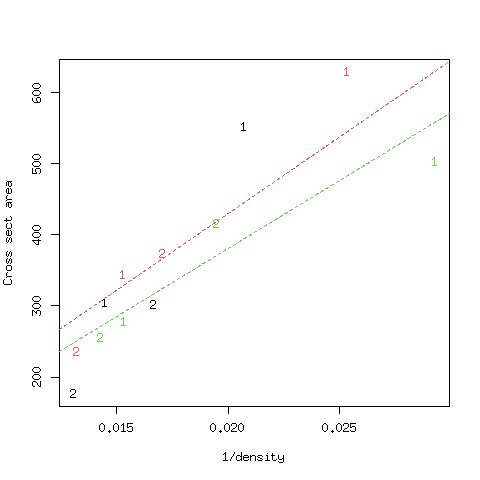
\includegraphics[width=0.9\textwidth]{C19391951/strainxnut.png}
  \caption{Plot of breed means for reciprocal of follicle density and fibre cross sectional area from Carter(1939)~\cite{cart:39}. The red line is a linear regressions  with zero intercept fitted to strain x age means for the high nutrition group. The green line is a linear regressions with zero intercept fitted to strain x age means for the Low nutrition group.}
  \label{fig:oldcart1}
\end{figure}

%\end{document}


The High nutrition group has a $k$ (ie slope of regression) of 21481, while the Low nutrition group has a $k$ of 19059. This is in the direction noted previously, ie higher $k$ values indicate better nutrition, but the difference is not large. 
The High nutrition group has a $k$ (ie slope of regression) of 21481, while the Low nutrition group has a $k$ of 19059. This is in the direction noted previously, ie higher $k$ values indicate better nutrition, but the difference is not large. There is no record of level of feeding in the High and Low nutrition groups, but the bodyweight differences were large, and the fleece weight differences were large. We can at least conclude tthat the difference in $k$ is due to nutrition, because the design is randomised. 

There is a lot of variation around the regressions in Figure~\ref{fig:oldcart1}. We look into this with an analysis of variance of the $k$ values for Strain x Age x Nutrition combinations, as follows
\begin{verbatim}
            Df   Sum Sq  Mean Sq F value Pr(>F)  
Strain        1 30539076 30539076  11.695 0.0188 *
NutPlane      1 32654244 32654244  12.505 0.0166 *
Age           2 20132088 10066044   3.855 0.0971 .
NutPlane:Age  2 49939448 24969724   9.562 0.0196 *
Residuals     5 13056235  2611247                 
---
Signif. codes:  0 ‘***’ 0.001 ‘**’ 0.01 ‘*’ 0.05 ‘.’ 0.1 ‘ ’ 1
\end{verbatim}
There is an interaction between NutPlane and Age.  This is summarized by the following table of means
\begin{verbatim}
 NutPlane:Age 
        Age
NutPlane 1     2     3    
    High 23858 23640 17629
    Low  15828 19846 19556
\end{verbatim}
Something happened to the difference between High and Low NutPlanes at Age 3 - the effect is reversed. The differences in $k$ at Ages 1 and 2 are much larger and more in line with those found in the Daly and Carter experiments. 
 We will never find out what happened at Age 3, but both Strains in the High NutPlane group suddenly became finer, while both Strains in the Low Nutplane group increased slightly in diameter? 

There is a further old unpblished study by Thompson and Carter(1952)~\cite{thom:52}. The result sheets are shown in Figures~\ref{fig:thomcart1},~\ref{fig:thomcart2}, and~\ref{fig:thomcart3}
%\documentclass{article}
%\usepackage{graphicx,subfigure}
%\begin{document}

\begin{figure}[h]
  \centering
   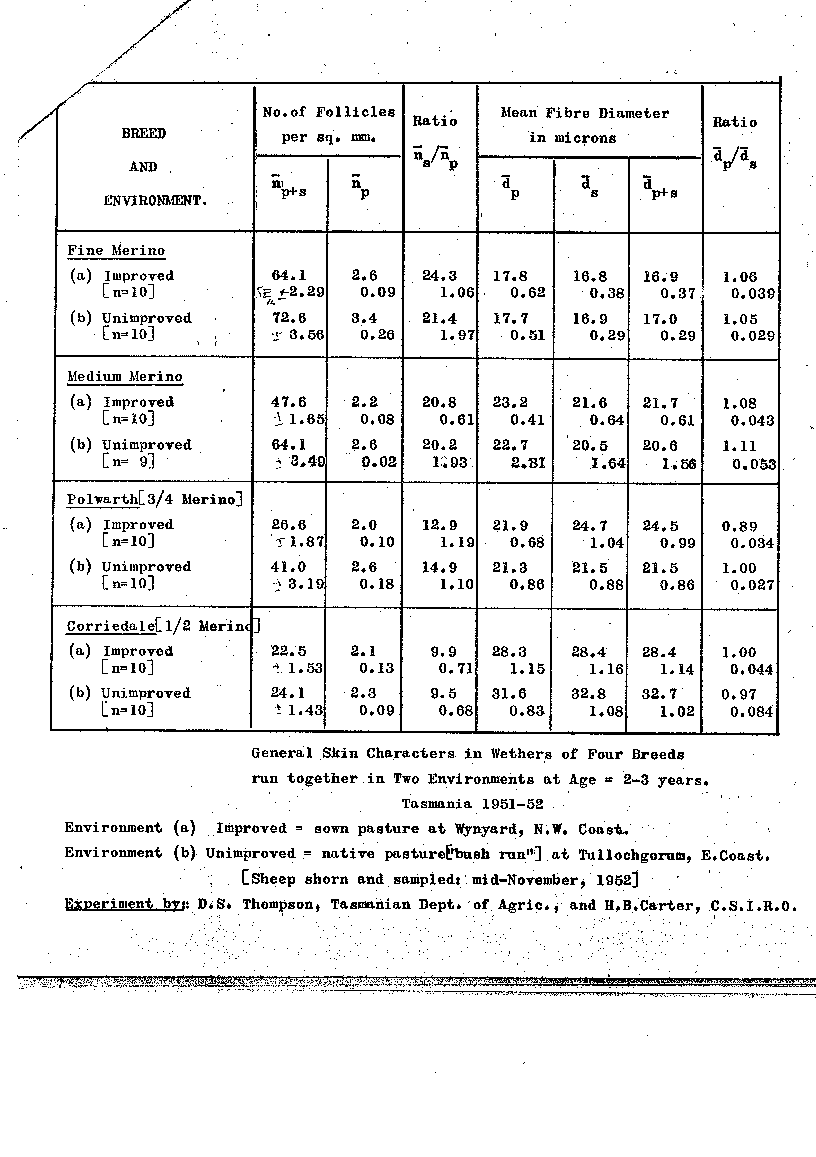
\includegraphics[width=1.1\textwidth]{carter51a.png}
  \caption{Data from an old nutritional experiment obtained from Dr Carter}
  \label{fig:thomcart1}
\end{figure}

%\end{document}


%\documentclass{article}
%\usepackage{graphicx,subfigure}
%\begin{document}

\begin{figure}[h]
  \centering
   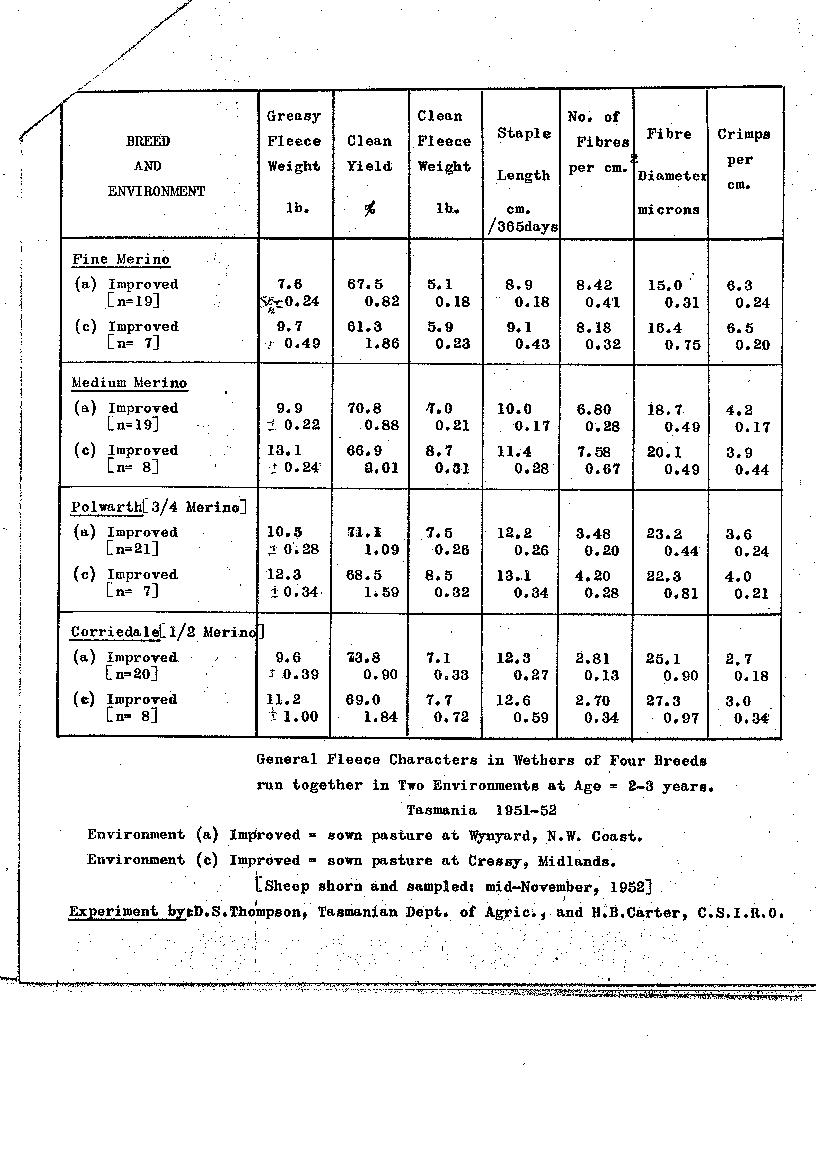
\includegraphics[width=1.1\textwidth]{carter51b.png}
  \caption{Data from an old nutritional experiment obtained from Dr Carter}
  \label{fig:thomcart2}
\end{figure}

%\end{document}


%\documentclass{article}
%\usepackage{graphicx,subfigure}
%\begin{document}

\begin{figure}[h]
  \centering
   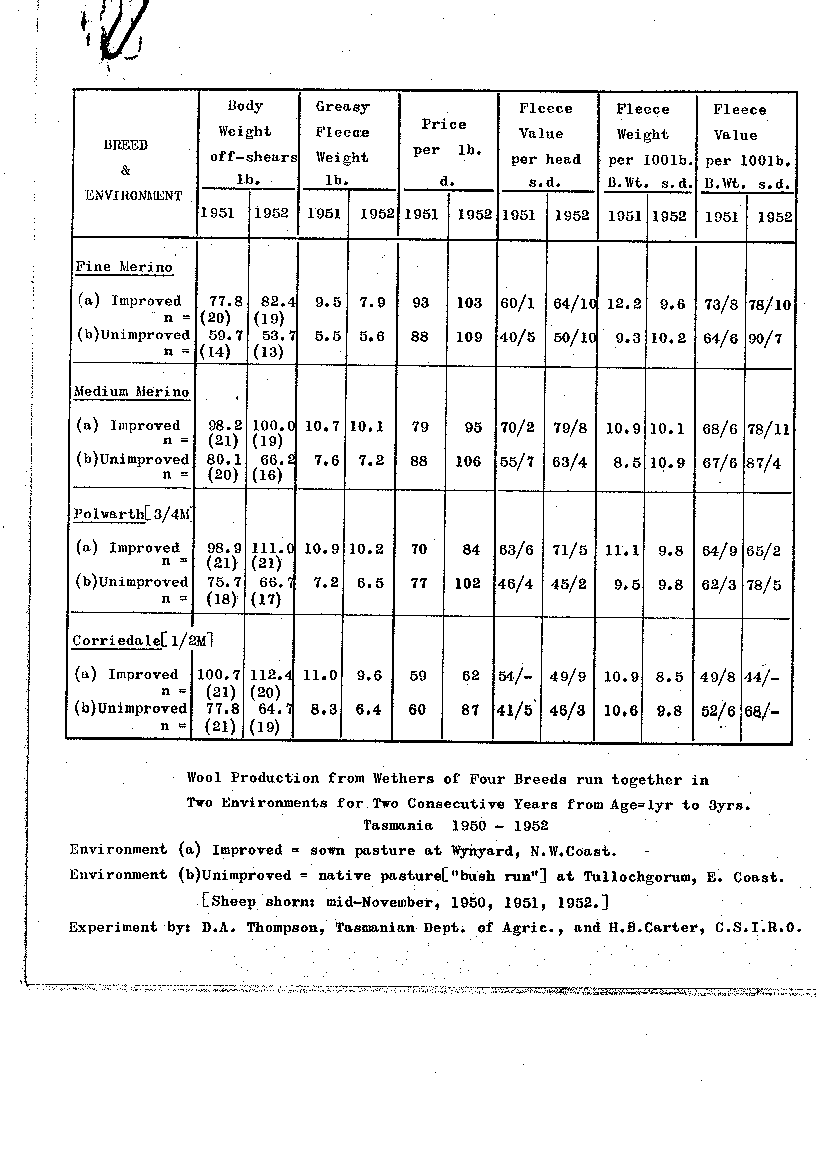
\includegraphics[width=1.1\textwidth]{carter51c.png}
  \caption{Data from an old nutritional experiment obtained from Dr Carter}
  \label{fig:thomcart3}
\end{figure}

%\end{document}


The plot of reciprocal density against cross sectional area for these data is shown in Figure~\ref{fig:cart52}
%\documentclass{article}
%\usepackage{graphicx,subfigure}
%\begin{document}

\begin{figure}[h]
  \centering
   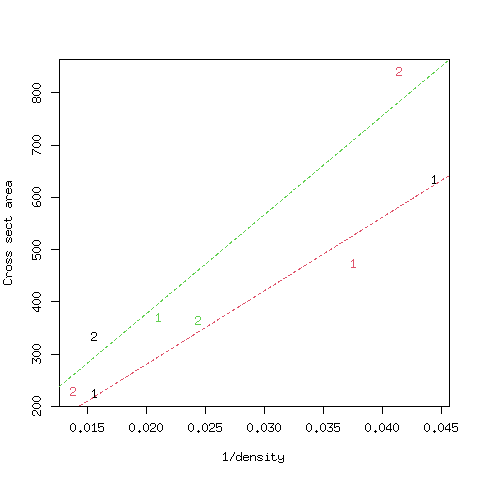
\includegraphics[width=1.1\textwidth]{C19391951/breedxpasture.png}
  \caption{Plot of reciprocal density against crosss sectional area for data from Thompson and Carter(1952)~\cite{thom:52}. Red line is regression through origin for the Improved Pasture group. Green line is regression through origin for the Unimproved Pasture group.}
  \label{fig:cart52}
\end{figure}

%\end{document}


This plot is interesting. The unimproverd pasture has a higher $k$ value ( green line) than the improved pasture (red line). The difference between pasture types in significant , as shown by the following analysis of variance of means
\begin{verbatim}
            Df   Sum Sq  Mean Sq F value Pr(>F)
Breed        3 36749637 12249879   7.708 0.0637 .
Pasture      1 25173778 25173778  15.840 0.0284 *
Residuals    3  4767746  1589249
---
Signif. codes:  0 ‘***’ 0.001 ‘**’ 0.01 ‘*’ 0.05 ‘.’ 0.1 ‘ ’ 1
\end{verbatim}
The residual is actually the interaction sum of squares, but it would not seem there is any interaction between Breeds and Pastures, as in the following set of  means for $k$ the difference betwen Improved and Unimproved Pasture is in the same direction for all Breeds
\begin{verbatim}
 Breed:Pasture
            Pasture
Breed        Improved Unimproved
  Corriedale 14253    20240
  FineMerino 14379    16479
  MedMerino  17604    21364
  Polwarth   12540    14885
\end{verbatim}
We can only suppose that either the unimproved pasture was actually 'better' than the improved, or that some other factor is involved. The two Pastures were at different locations.


\clearpage
\subsubsection{Trangie Flc+ and Flc- lines feeding experiment}
Williams and Winston(1987)~\cite{will:87} conducted a feedsing experimant in which ewes from the Trangie Flc+ and Flc- selection lines were randomly allocated to two groups fed a High and  Low ration for a period of 100 days. Follicle density and fibre cross sectional area were measured at the end of the treatment period. A plot of reciprocal density against cross sectional area is shown in Figure~\ref{fig:ww}
%\documentclass{article}
%\usepackage{graphicx,subfigure}
%\begin{document}

\begin{figure}[h]
  \centering
   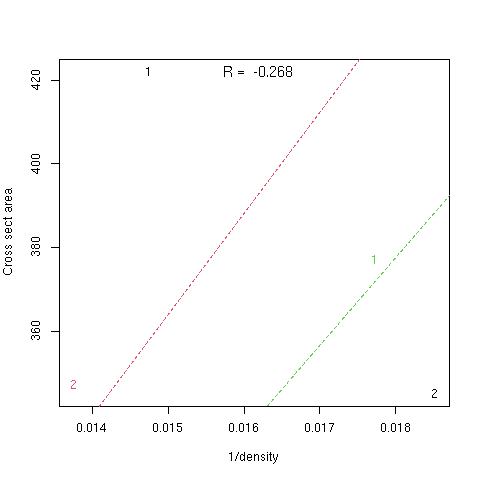
\includegraphics[width=1.1\textwidth]{WW1987/ww.png}
	\caption{Data from Williams and Winston(1987)~\cite{will:87} showing reciprocal density and cross sectional area for Trangie Flc+ and Fls - sheep under High and Low levels of feeding. Red line is regression thru origin for High level Diet, green line is regression thru origin for Low level of diet}
  \label{fig:ww}
\end{figure}

%\end{document}


This looks like an insignificant result but the range of variation is tiny compared to previous graphs and there are only 2 points, one from Flc+ and one fron Flc-, for each diet level. The two slopes were  24268 for High Diet and 20976 for Low Diet, so they are within the ranges of previous datasets. An analysis of variance of $k$ values gives 
\begin{verbatim}
            Df   Sum Sq  Mean Sq F value Pr(>F)
Line         1 68774420 68774420  24.987  0.126
Diet         1  8857061  8857061   3.218  0.324
Residuals    1  2752389  2752389               
\end{verbatim}
and the Line x Diet means were
\begin{verbatim}
 Line:Diet 
      Diet
Line   H     L    
  Flc+ 30125 25490
  Flc- 20173 18856
\end{verbatim}
so the Line difference is large and significant, the Diet difference is small and not significant.

We have to conclude $k$ can be changed by intense selection for one trait ( in this case fleece weight). We know that $k$ is not just how much the animal eats, but something like nutritional status of a skin area or a follicle group.  That could easily be influenced by all sorts of genetic mechanisms in the skin as well as by overall nutritional status.


\clearpage
\subsubsection{CSIRO selection lines}
The experiments reported by Turner,Brooker and Dolling (1970)~\cite{turn:70} are single character selection lines with pairs of lines selecte up and down for the following traits - Bodyweight, Density, Staple Length, CWW per head , Wrinkle, Fibre Diameter, CWW per unit area, and Clean Scoured Yield of wool. Figures~\ref{fig:kfs2} and ~\ref{fig:kfs3} show plots of the $k$ values of sheep born in years 1947 to 1970.
%\documentclass{article}
%\usepackage{graphicx,subfigure}
%\begin{document}

\begin{figure}[h]
  \centering
   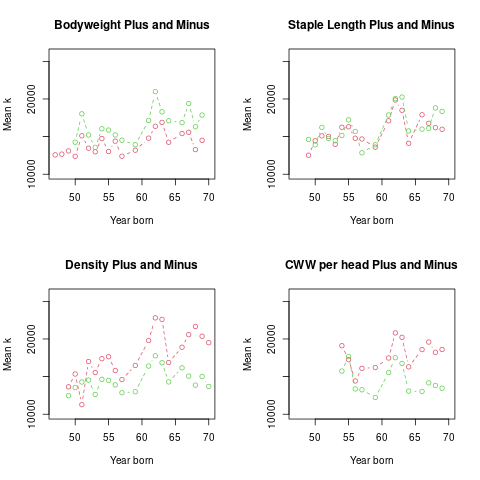
\includegraphics[width=1.4\textwidth,height=1.7\textwidth]{ab1fs/kfs2.png}
	\caption{Data from Turner, Brooker, and Dolling (1970)~\cite{turn:70} showing the mean $k$ value for sheep born in years 1947 to 1970  of four single trait selection lines with selection up and down for eight wool traits. Red lines are Plus selection. Green lines are Minus selection}
  \label{fig:kfs2}
\end{figure}

%\end{document}


%\documentclass{article}
%\usepackage{graphicx,subfigure}
%\begin{document}

\begin{figure}[h]
  \centering
   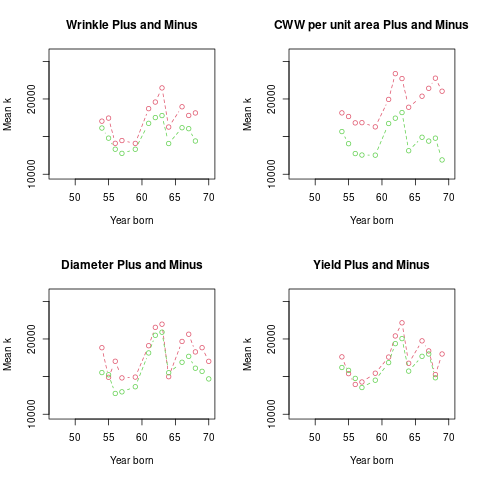
\includegraphics[width=1.4\textwidth,height=1.7\textwidth]{ab1fs/kfs3.png}
	\caption{Data from Turner, Brooker, and Dolling (1970)~\cite{turn:70} showing the mean $k$ value for sheep born in years 1947 to 1970  of four single trait selection lines with selection up and down for eight wool traits. Red lines are Plus selection. Green lines are Minus selection}
  \label{fig:kfs3}
\end{figure}

%\end{document}


The result is clearcut. Density and diameter (which make up $k$) show a small response, as does bodyweight ( because surface area contributes to density). CWW per head and per unit area show a larger response in $k$ because they are density and diameter together, ignoring length. Length, wrinkle, and yield are unrelated to $k$, although there might be a small change in $k$ in the wrinkle plus and minus lines. CWW per unit area is just $k$ with length added.

So the whole thing is purely physical, $k = ND$ being the definition of $k$. It sheds no light on our interpretation of $k$ as skin nutritional status. There is , however , considerable year to year fluctuation in $k$ within all selection lines.  This fluctuation reflects yearly shifts in pasture quality and thus epresents the environmental sensitivity of $k$.   The difference between largest and smallest $k$ value is shown for each line in Table~\ref{tab:lineranges}.
% latex table generated in R 4.0.4 by xtable 1.8-4 package
% Sun Dec 12 20:45:26 2021
\begin{table}[ht]
\label{tab:lineranges}
\centering
\caption{Difference between largest and smallest $k$ value for each of 8 single character selection lines}
\vspace{0.1in}
\begin{tabular}{rr}
  \hline
 Line & Range of $k$ \\ 
  \hline
BwtPlus & 4509.70 \\ 
  BwtMinus & 7404.50 \\ 
  DensPlus & 11528.80 \\ 
  DensMinus & 5310.40 \\ 
  LengthPlus & 7333.10 \\ 
  LengthMinus & 7406.30 \\ 
  CWWPlus & 6383.40 \\ 
  CWWMinus & 5431.10 \\ 
  WrinklePlus & 7372.20 \\ 
  WrinkleMinus & 5024.20 \\ 
  DiamPlus & 7139.40 \\ 
  DiamMinus & 8137.50 \\ 
  CWWperuaPlus & 7072.10 \\ 
  CWWperuaMinus & 6296.10 \\ 
  YieldPlus & 8188.30 \\ 
  YieldMinus & 6501.90 \\ 
   \hline
\end{tabular}
\end{table}


Most of the ranges are around 5000-7000 but the Density Plus Line has a range of 11000. It may be that having a high Density makes sheep more responsive in Diameter to seasonal changes. 

\subsubsection{Quantitative genetic analysis of variation in $k$ within a Merino flock}
We have a modest amount of CSIRO data (820 sheep) in which fibre diameter and follicle density were measured on skin sections from a pedigreed Merino sheep flock.  This permits a quantitative genetic analysis of variation in $k$ among animals within a flock. We obtain the following estimates of heritable and non-heritable variance of $k$
\begin{verbatim}
Proportion of phenotypic var/covariance partitioned by DME:
 to each component (OLS-b):

         Trait Estimate StdErr CI95lo CI95hi
VarE(I)      k    0.798  0.029  0.741  0.855
VarG(Ia)     k    0.202  0.029  0.145  0.259
VarP(I)      k    1.000  0.000  1.000  1.000
\end{verbatim}
So the heritability of $k$ is not zero but is only 0.2, so 80 percent of the variance is non-heritable. That goes along with $k$ being mostly a skin nutritional status indicator.

We can also look at how $k$ is correlated with other variables
\begin{verbatim}
         Traitpair Estimate StdErr  CI95lo CI95hi
VarE(I)      k:Cww  -0.0108 0.0394 -0.0880 0.0663
VarG(Ia)     k:Cww   0.4495 0.1002  0.2531 0.6460
VarP(I)      k:Cww   0.0822 0.0240  0.0351 0.1293

         Traitpair Estimate StdErr CI95lo CI95hi
VarE(I)      k:Bwt  -0.1057 0.3619 -0.815 0.6036
VarG(Ia)     k:Bwt  -0.0521 0.1181 -0.284 0.1794
VarP(I)      k:Bwt  -0.0480 0.0611 -0.168 0.0717

         Traitpair Estimate StdErr CI95lo CI95hi
VarE(I)     k:Stal  -0.0947 0.0662 -0.225 0.0351
VarG(Ia)    k:Stal   0.0130 0.0945 -0.172 0.1982
VarP(I)     k:Stal  -0.0565 0.0336 -0.122 0.0094
\end{verbatim}
So there is a genetic correlation with Cww, and not much correlation of any type with Bwt or Staple Length. The positive correlation with Cww is just a reflection of the fact that cross sectional area is part of Cww, and also part of $k$. So there is nothing there to suggest that our interpretation of $k$ as skin nutritional status  is questionable. Remember that Staple Length and Cww are not point measures; they are integrations of the preceding year of wool growth.  We are viewing $k$ as an instantaneous measure of skin status, not an integrated measure during development.

\clearpage
\subsubsection{Staple diameter profile data}

..............
This section is not as definitive as I originally thought
It needs to be rewritten
There are only density measurements at the time of the tenth diameter reading along the profile. 
This limits what we can do with these data.
..................

Varying {\em check} is what makes staple diameter profiles. Data from Jackson and Downes (1979)~\cite{jack:79} has sheep from  4 single character selection lines (L+, L-, D+, D-). There were 5 sheep from each selection line, and 2 staples per sheep. All sheep were rams born in 1972. Each staple was divided into 10 equal length segments, and the mean fibre diameter of each segment was measured with the liquid scintillation counting technique (Downes et al 1975)~\cite{down:75}. Each staple represented wool growth from weaning in January 1973 to hogget shearing in February of 1974. The changes in diameter for each selection line are shown in Figure~\ref{fig:dproflines} which is copied from the paper
%\documentclass{article}
%\usepackage{graphicx,subfigure}
%\begin{document}

\begin{figure}[h]
  \centering
   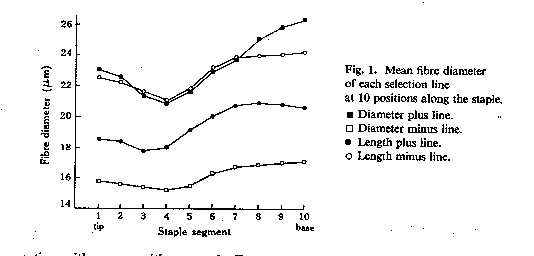
\includegraphics[width=1.0\textwidth]{dproflines.png}
  \caption{Mean diameter of each selection line at 10 positions along the staple. Taken from Jackson and Downes (1979)~\cite{jack:79}}
  \label{fig:dproflines}
\end{figure}

%\end{document}



In trying to use these data to study the {\em check} effect we need to be aware of the changes that are occurring as the wool growth proceeds from segment 1 to segment 10. At segment 1 the sheep are weaners, by segment 10 they are hoggets of about 18 months of age, and almost mature. Over this period the sheep increase in body weight and surface area, but decrease in follicle density. At the same time segment 1 is end of Summer, the pastures in Armidale then go into an Autumn/Winter decline, so segments 3,4, and 5 represent the poorest nutrition, and there is then an increase in pasture quality as we go into Spring and Summer up to segment 10.

So several things are altering simultaneously along the profiles.  They are all variations in degree of {\em check}, but by various mechanisms.

We first examine  a plot of reciprocal density against cross sectional area estimated from diameter of staple segment 10, which is at the same time as the density measurement. Figure~\ref{fig:sdpArecN} shows a separate regression line for each selection line (D+, D-, L+, L-).
%\documentclass{article}
%\usepackage{graphicx,subfigure}
%\begin{document}

\begin{figure}[h]
  \centering
   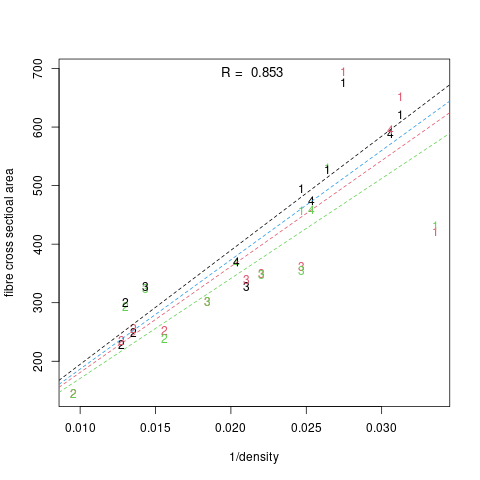
\includegraphics[width=1.1\textwidth]{SDP/sdpArecN.png}
  \caption{Plot of reciprocal density against cross sectional area of tenth staole segment for data from Jackson and Downes (1979)~\cite{jack:79}. Regression lines are through the origin. Black is D+ Line, red is D- Line. Green  is L+ Line. Blue is L- Line} 
  \label{fig:sdpArecN}
\end{figure}

%\end{document}


The data show a high correlation with some points from the D+ Line ( labelled '1' on the graph) being deviant than the remainder. The mean slopes for each line were
\begin{verbatim}
 Family 
       D+    D-    L+    L-
    19478 18094 17074 18668
rep    10    10    10     6
\end{verbatim}
An analysis of variance of $k$ values shows that Lines  and Sheep within Line varied significantly
\begin{verbatim}
Analysis of Variance Table

Response: k
             Df    Sum Sq  Mean Sq F value    Pr(>F)    
Line          3  30149810 10049937  57.925 1.906e-09 ***
Line:Sheep   14 311176471 22226891 128.110 4.477e-15 ***
Residuals    18   3122968   173498                      
---
Signif. codes:  0 ‘***’ 0.001 ‘**’ 0.01 ‘*’ 0.05 ‘.’ 0.1 ‘ ’ 1
\end{verbatim}
So the $k$ values ( slopes) of the 4 Lines are significantly different. What will be interesting will be to see whether these $k$ values correlate with the staple diameter profiles. Figure~\ref{fig:d10md4xk} shows a positive relationship between $k$ and $D10-D4$ with a correlation of 0.62
%\documentclass{article}
%\usepackage{graphicx,subfigure}
%\begin{document}

\begin{figure}[h]
  \centering
   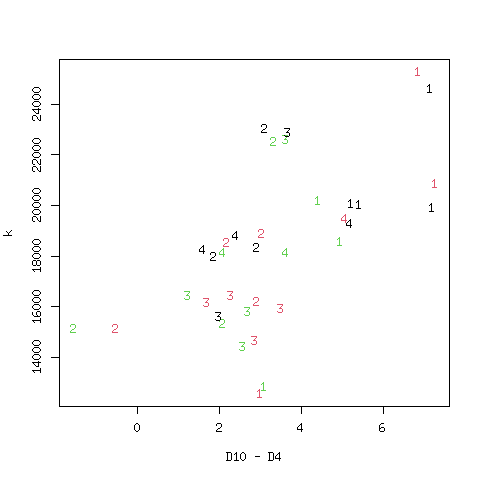
\includegraphics[width=1.1\textwidth]{SDP/d10md4xk.png}
  \caption{Plot of difference between D10 and D4 against $k$ value for individual sheep x replicate staple data from Jackson and Downes (1979)~\cite{jack:79}}
  \label{fig:d10md4xk}
\end{figure}

%\end{document}


So a larger $k$ means a more responsive diameter profile, or the reverse; a more responsive diameter profile leads to a larger end segment diameter and a larger end segment $k$. We are unable to sort out causation here, because we do not have densities ( and therefore $k$'s) at the first nine staple segments.

We can see whether the Line means show the same relationship as Figure~\ref{fig:d10md4xk} by plotting them in Figure~\ref{fig:d10md4xklm}
%\documentclass{article}
%\usepackage{graphicx,subfigure}
%\begin{document}

\begin{figure}[h]
  \centering
   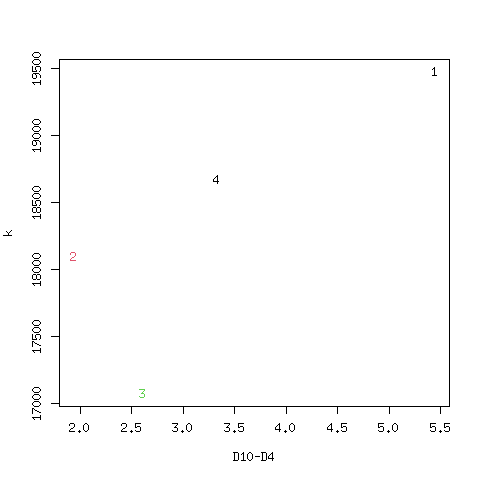
\includegraphics[width=1.1\textwidth]{SDP/d10md4xklm.png}
  \caption{Plot of Line means for difference between D10 and D4 against $k$ value for data from Jackson and Downes (1979)~\cite{jack:79}}
  \label{fig:d10md4xklm}
\end{figure}

%\end{document}


The relationship is still positive, and in this case the correlation among Line means is $0.79$. So whatever applies to Sheep applies to Line means also.

\clearpage
\subsection{Defining {\em check} by relating it to fibre diameter}
We have defined {\em check} at time $i$ $C_{i}$ as follows
\begin{displaymath}
 C_{i} = \frac{A_{B} - A_{i}}{A_{B}}
\end{displaymath}
which is just the fractional change in cross sectional area. This definition implies a linear relationship between $C$ and $A$, as shown in Figure~\ref{fig:checkdef}
%\documentclass{article}
%\usepackage{graphicx,subfigure}
%\begin{document}

\begin{figure}[h]
  \centering
   \includegraphics[width=1.0\textwidth]{checkdef/checkdef.png}
	\caption{Two relationships between check (C) and cross sectional area (A) implied by defining check as $C = \frac{A_{B} - A}{A_{B}}$. For the redline $A_{B}$ is set to 1256.6 (40 microns diameter), and this corresponds to zero check. For the green line $A_{B}$ is set to 706. (30 microns diameter), and this corresponds to zero check. Both lines intersect the X-axis at (1,0)}
  \label{fig:checkdef}
\end{figure}

%\end{document}


In Figure~\ref{fig:checkdef} the Y-axis intercept is $A_{B}$ and the slope is $-A_{B}$. 

We could define a curved relationship, such as an exponential decay function. This would make the rate of decay ( ie check) proportional to the value of $A$, so that a sequence of checks would encounter diminishing responses in $A$. 

The linear definition has fibres with a larger $A_{B}$ respond more to a given check than fibres with a smaller $A_{B}$, and that is what we observe,  but the rate of response does not change along a sequence of checks, so we get a straight line relationship. 

We have assumed the $A_{B}$ is known. This is not the case. The only way one could directly obtain $A_{B}$ would be estimation from dermal papilla cell counts. We would need a calibration of DPC counts to $A_{B}$. We do not have such a calibration. We only have a relationship of DPCC to checked $A$ at an unknown level of check. To get anywhere we need an independent measure of check.

\subsection{Measuring {\em check}}
Our hypothesis is that check has two components
\begin{description}
\item[developmental component] the amount of check is directly proportional to density $(N)$. The more fibres/follicles there are to share resources, the greater the check.
\item[nutritional component] the amount of check is inversely proportional to the nutritional status of the skin. The less resources there are to share among a given number of follicles, the greater the check.
\end{description}

The developmental component has been well studied , particularly in relation to birthcoats and prenatal check. Prenatal check is attributed to the sudden increase in number of secondary derived (Sd) follicles which occurs just before birth.

The skin resources component is elusive. We have attempted in the data analyses from nutritional and other experiments to show that $k$ ( the constant of a hyperbolic equation relarting $A$ to $N$)  is at least an indicator of skin nutritional status - high $k$ indicating more skin nutrients.

So what our hypothesis implies  about check $C$ is
\begin{displaymath}
C \propto \frac{N}{k}
\end{displaymath}
but this has problems. $k$ is the sum of the areas of all fibres in a unit area, which can be written $N \overline{A}$, so $C$ becomes $\frac{N}{N \overline{A}}$, which is $\frac{1}{\overline{A}}$. That is true - the smallest fibres have the largest check, but it does not tell us anything useful, and the logic is circular.

We need to take a different approach.  Go back to the original Carter(1968) graph (Figure~\ref{fig:carternxc}) and draw the family of hyperbolas implied by a set of $k$ values. The result is shown in Figure~\ref{fig:hypfam}
%\documentclass{article}
%\usepackage{graphicx,subfigure}
%\begin{document}

\begin{figure}[h]
  \centering
   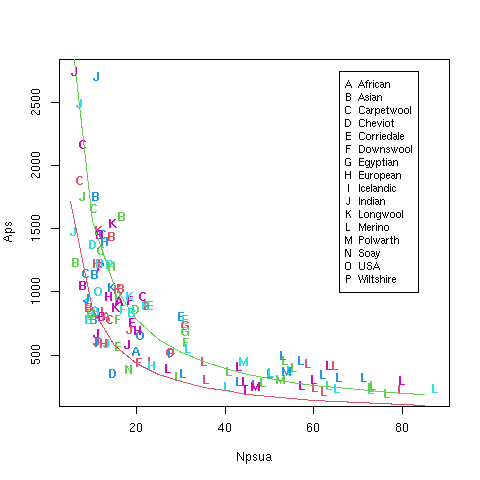
\includegraphics[width=0.9\textwidth]{carter68/carter68withk.png}
  \caption{Plot of breed means for follicle density and fibre cross sectional area from Carter(1968)~\cite{cart:68}. Red line shows points with a $k$ value of 8600, green line a $k$ value of 15600.}
  \label{fig:hypfam}
\end{figure}

%\end{document}


The red and green 'lines of equal $k$ value' are quite close, but follow the data points closely.  We have got it right - $k$ reflects the position of the hyperbola - ie its distance ifrom the origin along the 45 degree axis of the hyperbola.

We need to take a closer look at how one parameterizes hyperbolic data.  THere is a way of transforming data to hyperbolic coordinates. For a point (x,y) in one quadrant with CFartesian coordinates ( ie as in the plot of $N$ against $A$), the corresponding hyperbolic coordinates plotted on a Cartesian quadrant are defined as
\begin{eqnarray*}
u & = & \ln{\sqrt{\frac{x}{y}}} \\
v & = & \sqrt{xy}
\end{eqnarray*}
THe inverse mapping is 
\begin{eqnarray*}
x & = & v \exp{u} \\
y & = & v \exp{-u}
\end{eqnarray*}
So $v$ is $sqrt{k}$, which is just the geometric mean of $x$ and $y$, but $u$ is something new. $u$ is called the hyperbolic angle to $(x,y)$ , and it is a measure of how far along the curves of equal $k$ the point $(x,y)$ is located. 

Figure~\ref{fig:hypcoord} plots u against v for the Carter(1968) data.
%\documentclass{article}
%\usepackage{graphicx,subfigure}
%\begin{document}

\begin{figure}[h]
  \centering
   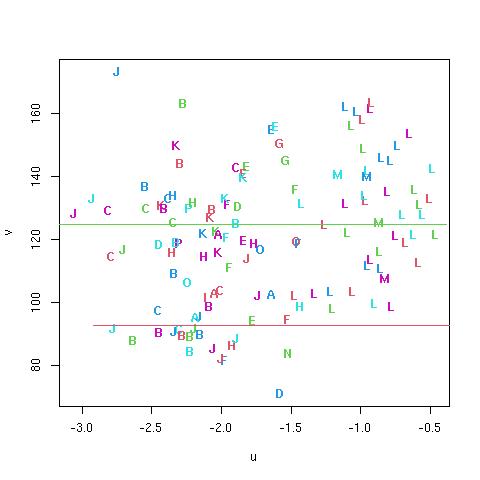
\includegraphics[width=0.9\textwidth]{carter68/hypcoordcarter68.png}
  \caption{Plot of breed means for hyperbolic coordinates $u$ and $v$ for data from Carter(1968)~\cite{cart:68}. Red line shows points with a $k$ value of 8600, green line a $k$ value of 15600.}
  \label{fig:hypcoord}
\end{figure}

%\end{document}


We see that $u$ puts Merino sheep ( coded L) to the far right side of the graph, ie to high values of $u$, and puts Indian breeds ( hair sheep coded J) to the far left. So the positioning along the hyperbola has been transformed to the $u$ coordinate , ie to a linear scale. The red and green lines for $k=8600$ and $k=15600$ are seen to correspond to $v$. It would seem that $u$ and $v$ are independent. $A$ and $N$ are certainly not independent.

Can we arrive at a biological interpretation of $u$, and is it useful? Yes $u$ is $\ln{\sqrt{\frac{N}{A}}}$. So $u$ is the variable that describes the process in the Moore dermal papilla cell model whereby a small number of dermal papilla cells per initiating follicle leads to both a larger number of initiating follicles $(N)$ and to smaller fibres $(A)$. This is expressed by $\frac{N}{A}$. The rest ( ie the square root and log) are just scaling. 

If $k=v^{2}$ is all effects on $A$ except density, and $u$ is the  Moore model efffect of $A$ on density, there remains the issue of 'can we get at $A_{B}$ ( the maximum value of $A$ determined by dermal papilla cell number? The answer is that $A_{B}$ is the value of $A$ at $N=1$ ( ie where there are no other fibres).  Given $k = N A$, if we substitute $N=1$ we get $A_{B} = k$. So $k$ is both 'non-density effects on $A$' and $A_{B}$. How can it be both? Well, 2 things can be numerically equal without being the same, but that begs the question. We need to investigat e the following
\begin{itemize}
\item is the (N,A) relationship really an hyperbola, and is it centred on (0,0)? THe (1/N,A) plots being linear supports it being an hyperbola. 
\item an alternative is a negative exponential curve. Exponential decay curves intersect the Y axis but are asymptotic to the X axis. In this case $A_{B}$ would be the point of intersection with the Y axis. So is the check process like radioactive decay?
\item can we gain any understanding fromn other physical 'laws' which are hyperbolic - eg Ohms law, Boyles law. Anywhere 2 variates are multiplied leads to an hyperbolic 'law'. 
\item our graphs of the (N,A) function look regular - but that is because we have scaled the axes. If we plotted with equal units for N and A the hyperbolic curve would not have its axis at 45 degrees but the origin would still be (0,0) so long as we plotted $N A = k$. If we plotted $(N-h) (A-j) = k$ the origin would be at (h,j). Not sure if we could determine whether a particular set of points had origin (0,0), but the regressions of $A$ on $1/N$ being thru the origin suggest that the origin is indeed (0,0).

\end{itemize}

\clearpage
\section{Discussion}

............................  this came from poisson.tex ..... ignore it
Our thesis is that most of the variation in diameter between fibres within a sheep is controlled by a random sampling of dermal papilla cell numbers forming aggregates. That is , it is not controlled at all, it is chance variation. We emulate this with sampling from a Poisson distribution.

However there is a small amount of fibre diameter variation that is due to systematic differences in dermal papilla cell number between follicle types (Pc, Pl, So, Sd) within a sheep. This variation is under genetic control, and is what is responsible for skewed within sheep fibre diameter distributions. We have ben able to show that one can simulate fibre diameter distributions with skewness or bimodality, simply by allocating more dermal papilla cells to the earliwer forming follicle types (Pc, Pl, So).

It may be that instead of making follicle types, the most realistic strategy may be to allocate dermal papilla cell numbers to follicles according to their time of initiation. The effect on diameter distribution would be similar. We have not tried this approach, but it may be more biologically meaningful.

............................................................
This bit might stay

While we are sure that dermal papilla cell number controls maximim or potential or base diameter ( actually cross sectional area) , all observed data are of {\em checked} diameter, ie what the follicles grow when they have to share a limited nutrient supply among all the follicles in a trio group.

\clearpage
\begin{thebibliography}{}

\bibitem{adel:02}
Adelson, FD. L. , Hollis, D. E. and Brown, G. H. (2002) Wool fibre diameter and follicle density are not specified simultaneously during wool follicle initiation. Aust. J. Agric. Res. 53:1003-1009

\bibitem{bogo:40}
 Bogolyubsky S.N. (1940) cited by Fraser A.S and Short B.F. (1960) The Biology of the Fleece. Animal Research Laboratories Technical Paper No 3. CSIRO Melbourne 1960.

\bibitem{cart:39}
Carter, H. B. Unpublished data personal communication. Refers to Marston, H. R. , Pierce, A. W. and Carter, H. B. (1939-42) which is unpublished.

\bibitem{cart:43}
Carter H.B. (1943) Studies in the biology of the skin and fleece of sheep. 1. The development and general histology of the follicle group in the skin of the Merino. 2. The use of tanned sheepskin in the study of follicle population density. 3. Notes on the arrangement, nomenclature, and variation of skin folds and wrinkles in the Merino. C.S.I.R. Bulletin No 164, Melbourne, 1943

\bibitem{cart:55}
Carter, H.B. (1955) The hair follicle group in sheep Animal Breeding Abstracts 23(2) 101-116

\bibitem{cart:68}
Carter,H.B. (1968) Comparative Fleece Analysis Data for Domestic Sheep. The Principal Fleece Staple Values of Some Recognised Breeds. Agricultural Research Council, 1968

\bibitem{chi:13}
Chi, W., Wu, E., and MOrgan, B.A. (2013) Dermal papilla cell number specifies hair size shape and cycling and its reduction causes follicular decline. Development 140(8):1676-1683

\bibitem{daly:55}
Daly, R.A. and Carter, H.B. (1955) The fleece growth of young Lincoln, Corriedale, Polwarth, and Fine Merino maiden ewes under housed conditions and unrestricted and progressively restricted feeding on a standard diet. Aust. J. Agric. Res. 6:476-513

\bibitem{daly:56}
Daly, R.A. and Carter, H.B. (1956) he fleece growth of young Lincoln, Corriedale, Polwarth, and Fine Merino maiden ewes grazed on an unimproved paspalum pasture. Aust. J. Agric. Res. 7:76-83

\bibitem{down:75}
Downes, A. M., Jackson, N. and Griffiths, D. A. (1975) Measurement of mean fibre diameter and colour quenching of wool samples by liquid scintillation spectrometry. 5th Int. Wool Text. Res. Conf. Aachen, Germany.

\bibitem{fras:60}
Fraser A.S and Short B.F. (1960) The Biology of the Fleece. Animal Research Laboratories Technical Paper No 3. CSIRO Melbourne 1960.

\bibitem{gord:08}
Gordon-Thompson, C., Botto, S.A., Cam, G.R., and Moore, G.P.H. (2008) Notch pathway gene expression and wool follicle cell fates. Aust. J. Exp. Agric. 48(5) 648-656

\bibitem{hard:56}
Hardy, M.H. and Lyne, A.G. (1956) The prenaltal development of wool follicles in Merino sheep. Aust. J. Biol. Sci. 9:423-441

\bibitem{jack:79}
Jackson, N. and Downes, A. M. (1979) The fibre diameter profile of wool staples from individual sheep. Aust. J. agric. Res. 30:163-171

\bibitem{jack:17}
Jackson, N. (2017) Genetics of primary and secondary fibre diameters and densities in Merino sheep. URL https://github.com/nevillejackson/atavistic-sheep/mev-rewrite/supplementary/genetic-parameters/psparam.pdf

\bibitem{jack:17a}
Jackson, N. (2017) Genetic relationship between skin and wool traits in Merino sheep. Part I Responses to selection and estimates of genetic parameters. URL https://github.com/nevillejackson/Fleece-genetics/tree/master/skinandfleeceparameters/ab3220/skinwool1.pdf

\bibitem{jack:17b}
Jackson, N. (2017) What are the defining characteristics of a primitive sheep relative to a Modern Merino sheep.  URL https://github.com/nevillejackson/atavistic-sheep/tree/master/mev-rewrite/supplementary/primitive/primitive.pdf

\bibitem{jack:18}
Jackson, N., Swan, P.G.S. and Watts, J.E. (2018) Questions regarding developmental control of fibre diameter and fibre length growth rate in sheep. URL https://github.com/nevillejackson/Fleece-biology/tree/master/diamlen/diamlen.pdf

\bibitem{jack:21}
Jackson, N. and Moore, G.P.M. (2021) Modelling trio group formation from a population of pre-papilla cells. Unfinished work.

\bibitem{jack:90}
Jackson, N., Maddocks, I.G., Lax, J., Moore, G.P.M. and Watts, J.E. (1990) Merino Evolution, Skin Characteristics, and Fleece Quality. URL https://github.com/nevillejackson/atavistic-sheep/mev/evol.pdf 

\bibitem{jack:18a}
Jackson, N. and Moore, G.P.H. (2018) R package {\em ppcell}. URL

\bibitem{madd:88}
Maddocks, I.G. and Jackson, N. (1988) Structural studies of sheep, cattle, and goat skin. CSIRO, Division of Aimal Production, Sydney.

\bibitem{metc:62}
Metcalf, J., Meschia, G., Hellegers, A., Prytowsky, H., Huchabee, W., and Barron, D.H. (1962) Observations on the growth rates and organ weights of fetal sheep at altitude and sea level. Quart. J. exp. Physiol. XLVII (4) 305-313

\bibitem{moor:84}
Moore G.P.M. and Jackson, N. (1984) An hypothesis implicating a founder cell population in the regulation of wool follicle formation and distribution in sheep skin. J. Embryol. Exp. Morph. 82 (Suppl), 259

\bibitem{moor:89}
Moore G.P.M., Jackson, N., and Lax, J. (1989) Evidence of a unique developmental mechanism specifying both wool follicle density and fibre size in sheep selected for single skin and fleece characters. Genet. Res. Camb. 53:57-62

\bibitem{moor:98}
Moore, G.P.M., Jackson, N., Isaacs, K., and Brown, G (1998) J. Theoretical Biology 191:87-94

\bibitem{rprog:13}
R Core Team (2013). R: A language and environment for statistical
  computing. R Foundation for Statistical Computing, Vienna, Austria.
  ISBN 3-900051-07-0, URL http://www.R-project.org/.

\bibitem{ryde:84}
Ryder, M. L. (1984) Medieval Sheep and Wool Types.  Agricultural History Review 32:14-28

\bibitem{ryde:68}
Ryder, M.L. and Stevenson, S.K.(1968) Wool Growth. Academic Press, London.

\bibitem{swan:21}
Swan, P. G., Jackson, N. and Moore, P, G. M. (2021) Dermal papilla cell counts and fibre diameter. URL  not there yet!

\bibitem{tapl:62}
Taplan, D.E., and Everitt, G.C. (1962) The influence of prenatal nutrition on postnatal performance of Merino lambs. Waite Agricultural Research Institute, University of Adelaide: 72-81
URL https://pdfs.semanticscholar.org/90b6/
db6e9763d25add182220c0b369023072d41b.pdf

\bibitem{thom:52}
Thompson, D.A. and Carter, H.B. (1952) Personal communication. Wool production from wethers of 4 breeds run together in two environments - improved pasture and unimproved pasture. Experiment conducted in Tasmania over years 1950-52

\bibitem{turn:70}
Turner, H.N., Brooker, M.G. and Dolling, C.H.S(1970) Response to selection in Australian Merino sheep. III Single character selection for high and low values of clean wool weight and its components. Aust. J. agric. Res. 21:955-984

\bibitem{watt:18}
Watts, J.E., and Jackson, N. (2018) Is collagen quantity and properties involved in wrinkle formation and/or in follicle development? URL https://github.com/nevillejackson/SRS-Merino/tree/master/supplementary/collagen/collagen.pdf

\bibitem{will:87}
Williams, A.J. and Winston, R.J. (1987) A study of the characteristics of wool follicle and fibre in Merino sheep genetically different in wool production. Aust. J. Agric. Res. 38:743-755

\bibitem{xavi:03}
Xavier, S.P., Gordon-Thomson, C. Wynn, P.C., McCullagh, P., Thomson, P.C., Tomkins, L., Mason, R.S., and Moore, G.P.M.(2003) Evidence that Notch and Delta expressions have a role in dermal condensate aggregation during wool follicle initiation. Experimental Dermatology, 22:656-681

\end{thebibliography}

\appendix
\section{Appendix}
The raw data are listed here for completeness
\end{document}
